%%%%%%%%%%%%%%%%%%%%%%%%%%%%%%%%%%%%%%%%%
% TMDEI Dissertation
% LaTeX Template
% Version 0.1 (Dec/2015)
%
% Adapted to TMDEI/ISEP style (Dec/2015) by
%  Nuno Pereira (nap@isep.ipp.pt) and
%  Paulo Baltarejo (pbs@isep.ipp.pt)
%
% Based on MastersDoctoralThesis Version 1.2 by Vel (vel@latextemplates.com) and
% Johannes Böttcher, downloaded from (21/11/15):
% http://www.LaTeXTemplates.com
%
% This template is originally based on a template by:
% Steve Gunn (http://users.ecs.soton.ac.uk/srg/softwaretools/document/templates/)
% Sunil Patel (http://www.sunilpatel.co.uk/thesis-template/)
%
% Template license:
% CC BY-NC-SA 3.0 (http://creativecommons.org/licenses/by-nc-sa/3.0/)
%
%%%%%%%%%%%%%%%%%%%%%%%%%%%%%%%%%%%%%%%%%
%----------------------------------------------------------------------------------------
%	PACKAGES AND OTHER DOCUMENT CONFIGURATIONS
%----------------------------------------------------------------------------------------

\documentclass[
11pt, % The default document font size, options: 10pt, 11pt, 12pt
%oneside, % Two side (alternating margins) for binding by default, uncomment to switch to one side (for drafting/reading purposes)
%openany, % Starts the chapter on the next page, even or odd (not recommended)
%english, % english for English;
portuguese,% for Portuguese; delete temporary files if you change language (e.g. 'make clean; make')
singlespacing, % Single line spacing, alternatives: onehalfspacing or doublespacing (for drafting/reading purposes)
%draft, % Uncomment to enable draft mode (no pictures, no links, overfull hboxes indicated)
%nolistspacing, % If the document is onehalfspacing or doublespacing, uncomment this to set spacing in lists to single
liststotoc, % Uncomment to add the list of figures/tables/etc to the table of contents (recommended)
%toctotoc, % Uncomment to add the main table of contents to the table of contents (not recommended)
parskip, % Add space between paragraphs (recommended)
%nohyperref, % Uncomment to not load the hyperref package (not recommended)
nohyperreflinkcolor, % hyperref links are not colored (comment to color links, for 
example to produce an electronic-only version)
headsepline, % Uncomment to get a line under the header
]{tmdei-style} % The class file specifying the document structure

\usepackage{tikz} % Required for creating graphics programmatically (can be removed if not used)
\usetikzlibrary{arrows.meta,positioning} % Used by the architecture diagram in Chapter 3

\usepackage{pgfplots} % Required for drawing high--quality function plots (can be removed if not used)
\pgfplotsset{compat=newest}

\usepackage[hidelinks]{hyperref} % no borders on links

%
% Citation style: authoryear-comp (Harvard-like), as recommended by the template
%
\usepackage[style=authoryear-comp,backend=biber]{biblatex} % Bibtex backend with the authoryear-comp citation style (authoryear citations, bibliography ordered alphabetically)

\addbibresource{mainbibliography.bib} % The filename of the bibliography

\makeglossaries % build the glossary

%----------------------------------------------------------------------------------------
%	THESIS INFORMATION
%----------------------------------------------------------------------------------------

% TODO: confirmar com o orientador que o título coincide com o submetido em Projetos@ISEP
\thesistitle{Assistente Conversacional Multilingue para Perguntas Médicas no Adhara QBank} % Your thesis title, this is used in the title, print it elsewhere with \ttitle

%\thesissubtitle{{[}Thesis Subtitle{]}} % Your thesis title, this is used in the title, print it elsewhere with \tsubtitle

\author{Francisco Reis} % Your name, this is used in the title page, print it elsewhere with \authorname

% TODO: confirmar a área de especialização (Cybersecurity and Systems Administration; Data Engineering; Software Engineering; Games, Graphics and Interactive Systems; Information and Knowledge Systems)
\subjectarea{Software Engineering} % Specialisation area, used in the title page, print it elsewhere with \areaname

\advisor{Nuno Silva} % Your advisors's (academic mentor) name, this is used in the title page, print it elsewhere with \advname

%\advisors{Dr. Jane \textsc{Smith} and Dr. Jake Smith} % In case you have multiple advisors and/or do not want to distinguish between advisor and co-advisor, use \advisors; if defined, will override \advisor

%\coadvisor{Dr. Jack \textsc{Smith}} % Your co-advisors's name, this is used in the title page, print it elsewhere with \coadvname (comment, if no co-advisor)

\supervisor{[Nome do Supervisor na Adhara]} % Your supervisor's (company, hosting institution mentor) name, this is used in the title page, print it elsewhere with \supname (comment, if no supervisor, or same as advisor)

%\supervisors{Dr. James \textsc{Smith} and Jace Smith} % In case you have multiple supervisors and/or do not want to distinguish between supervisor and co-supervisor use \supervisors; if defined, will override \advisor

%\cosupervisor{Dr. Jordan \textsc{Smith}} % Your co-advisors's name, this is used in the title page, print it elsewhere with \cosupname (comment, if no co-supervisor)

% if committeepresident is defined, will add the thesis committee to the front page (so only after the defense, in the final version)
%\committeepresident{Dr. Jonny Smith, Professor, DEI/ISEP} % Name of the president of the evaluation committee, print it elsewhere with \presidentname

%\committeemembers{Dr. Jaimie Smith, Professor, DEI/ISEP\\Dr. Jones Smith, Professor, DEI/ISEP\\Dr. Jagger Smith, Professor, DEI/ISEP} % Name of the evaluation committee members (up to four), print it elsewhere with \committee

\keywords{Modelos de Linguagem, Banco de Perguntas, Educação Médica, Geração Fundamentada em Contexto, Assistente Conversacional, Engenharia de Prompts} % Please define up to 6 keywords that better describe your work, print it elsewhere with \keywordnames

% TODO: confirmar os endereços web
\university{\href{https://www.isep.ipp.pt}{Instituto Superior de Engenharia do Porto}} % Your university's name and URL, this is used in the title page and abstract, print it elsewhere with \univname

\department{\href{https://www.dei.isep.ipp.pt}{Departamento de Engenharia Informática}} % Your department's name and URL, this is used in the title page and abstract, print it elsewhere with \deptname

\thesisdate{Porto, \today} % thesis date,  print it elsewhere with \tdate

\hypersetup{pdftitle=\ttitle} % Set the PDF's title to your title
\hypersetup{pdfauthor=\authorname} % Set the PDF's author to your name
\hypersetup{pdfkeywords=\keywordnames} % Set the PDF's keywords to your keywords

\begin{document}

%----------------------------------------------------------------------------------------
%	FRONT MATTER
%----------------------------------------------------------------------------------------

% Include the frontmatter of your thesis here
% we include the glossary here (frontmatter is included with \input, so this command is as if it was in main.tex)
%All acronyms must be written in this file.
% Só os acrónimos usados no texto com \gls{...} aparecem na lista.
\newacronym{LLM}{LLM}{\emph{Large Language Model}}
\newacronym{MCQ}{MCQ}{\emph{Multiple-Choice Question}}
\newacronym{RAG}{RAG}{\emph{Retrieval-Augmented Generation}}
\newacronym{DSR}{DSR}{\emph{Design Science Research}}
\newacronym{SLR}{SLR}{\emph{Systematic Literature Review}}
\newacronym{API}{API}{\emph{Application Programming Interface}}
\newacronym{GPU}{GPU}{\emph{Graphics Processing Unit}}
\newacronym{CPU}{CPU}{\emph{Central Processing Unit}}
\newacronym{VRAM}{VRAM}{\emph{Video Random Access Memory}}
\newacronym{TTFT}{TTFT}{\emph{Time To First Token}}
\newacronym{JSON}{JSON}{\emph{JavaScript Object Notation}}
\newacronym{RGPD}{RGPD}{Regulamento Geral sobre a Proteção de Dados}

\frontmatter % Use roman page numbering style (i, ii, iii, iv...) for the pre-content pages

\pagestyle{plain} % Default to the plain heading style until the thesis style is called for the body content

%----------------------------------------------------------------------------------------
%	TITLE PAGE
%----------------------------------------------------------------------------------------

\maketitlepage


%----------------------------------------------------------------------------------------
%	STATEMENT of INTEGRITY
%----------------------------------------------------------------------------------------
\integritystatement

%----------------------------------------------------------------------------------------
%	DEDICATION  (optional)
%----------------------------------------------------------------------------------------
%
%\begin{dedicatory}
%Dedicatória (opcional).
%\end{dedicatory}

%----------------------------------------------------------------------------------------
%	ABSTRACT PAGE
%----------------------------------------------------------------------------------------

\begin{abstract}

% Resumo na língua principal do trabalho (português), até 200 palavras.


No Adhara QBank, cada pergunta de escolha múltipla está associada a informação estruturada que vai além da explicação apresentada ao estudante durante a resolução do exame. Esta diferença pode deixar dúvidas por esclarecer, apesar de existirem dados relevantes na base de dados do item. Esta dissertação, desenvolvida em colaboração com a Adhara, concebe, implementa e avalia um assistente conversacional que responde a dúvidas sobre a pergunta em curso com base nessa informação.


O assistente foi concebido para interagir em várias línguas, responder apenas quando a informação do item sustenta a resposta e recusar questões fora do contexto disponível. A avaliação considera a correção e fidelidade das respostas, a capacidade de recusa, o desempenho e a utilidade percebida pelos utilizadores. A abordagem segue a metodologia \emph{Design Science Research}.

% TODO: completar com os resultados e conclusões principais no fim do trabalho.

\end{abstract}

\begin{abstractotherlanguage}
% Abstract in English (the work is written in Portuguese), about 200 words.


At Adhara QBank, each multiple-choice question is associated with structured information beyond the explanation shown to students while they answer an exam. This difference may leave questions unresolved even when relevant data are available in the item's database record. Developed in collaboration with Adhara, this dissertation designs, implements and evaluates a conversational assistant that answers questions about the current item using that information.


The assistant is designed to interact in multiple languages, answer only when the item's information supports a response, and refuse questions outside the available context. The evaluation considers answer correctness and faithfulness, refusal capability, performance and perceived usefulness. The approach follows the Design Science Research methodology.

% TODO: complete with the main results and conclusions at the end of the work.

\end{abstractotherlanguage}

%----------------------------------------------------------------------------------------
%	ACKNOWLEDGEMENTS (optional)
%----------------------------------------------------------------------------------------

\begin{acknowledgements}

% TODO: agradecimentos (opcional): orientador, supervisor na Adhara, família, amigos.

\end{acknowledgements}

%----------------------------------------------------------------------------------------
%	LIST OF CONTENTS/FIGURES/TABLES PAGES
%----------------------------------------------------------------------------------------

\tableofcontents % Prints the main table of contents

\listoffigures % Prints the list of figures

\listoftables % Prints the list of tables

% Descomentar quando existirem algoritmos / listagens de código no documento:
%\iflanguage{portuguese}{
%\renewcommand{\listalgorithmname}{Lista de Algor\'itmos}
%}
%\listofalgorithms % Prints the list of algorithms
%\addchaptertocentry{\listalgorithmname}
%
%\renewcommand{\lstlistlistingname}{List of Source Code}
%\iflanguage{portuguese}{
%\renewcommand{\lstlistlistingname}{Lista de C\'odigo}
%}
%\lstlistoflistings % Prints the list of listings (programming language source code)
%\addchaptertocentry{\lstlistlistingname}


%----------------------------------------------------------------------------------------
%	ACRONYMS
%----------------------------------------------------------------------------------------

\newcommand{\listacronymname}{List of Acronyms}
\iflanguage{portuguese}{
\renewcommand{\listacronymname}{Lista de Acr\'onimos}
}

%Use GLS
\glsresetall
\printglossary[title=\listacronymname,type=\acronymtype,style=long]

%----------------------------------------------------------------------------------------
%	DONE
%----------------------------------------------------------------------------------------

\mainmatter % Begin numeric (1,2,3...) page numbering
\pagestyle{thesis} % Return the page headers back to the "thesis" style

%----------------------------------------------------------------------------------------
%	MAIN BODY
%----------------------------------------------------------------------------------------

% Include the chapters of the thesis as separate folder for each chapter
% Uncomment the lines as you write the chapters

% Chapter 1
%
% NOTAS:
%  - Cada \textbf{[CITAR]} marca uma afirmação que precisa de referência verificada
%    (usa só fontes que confirmaste). Pesquisa por "CITAR" antes de entregar.
%  - Os pontos "a confirmar" dependem da revisão da literatura (Capítulo 2).
%
\chapter{Introdução} % Main chapter title
\label{chap:Chapter1} % For referencing the chapter elsewhere, use Chapter~\ref{Chapter1}


%-------------------------------------------------------------------------------
\section{Contexto e Motivação}
\label{sec:chap1_context}

Os bancos de perguntas de escolha múltipla (\glspl{MCQ}) são utilizados por estudantes de medicina para praticar e preparar exames. No Adhara QBank, um exame é composto por 40 perguntas, apresentadas ao estudante uma de cada vez. Enquanto responde a cada pergunta, o estudante tem acesso à vinheta clínica, às opções e à explicação disponibilizada pela plataforma, mas não necessariamente a toda a informação associada ao item.

Na base de dados do QBank, cada pergunta pode incluir, além do enunciado e da resposta, explicações gerais e por opção, dicas, informação-chave, conteúdo formativo e dados de catalogação. Esta informação estruturada pode ser relevante para aprofundar o raciocínio sobre a pergunta, mas não está toda diretamente acessível no ecrã de resposta. Os avanços em modelos de linguagem permitem explorar interfaces conversacionais para consultar esse conteúdo em linguagem natural. Num contexto médico e educativo, porém, é essencial que as respostas sejam fiáveis, adequadas à língua do estudante e limitadas à informação validada disponível para a pergunta \textbf{[CITAR]}.


%-------------------------------------------------------------------------------
\section{Definição do Problema}
\label{sec:chap1_problem}

Durante a resolução de uma pergunta no Adhara QBank, o estudante pode precisar de esclarecer aspetos que não são cobertos pela explicação apresentada no ecrã, por exemplo, porque uma determinada opção de resposta está errada. Embora a base de dados contenha informação adicional associada à pergunta, o estudante não dispõe de uma forma integrada de a consultar através de perguntas em linguagem natural. Recorrer a fontes externas ou a assistentes genéricos pode produzir respostas que não correspondem ao conteúdo validado do item ou que introduzem informação alheia ao contexto.

O problema abordado nesta dissertação é, assim, a dificuldade de obter esclarecimentos adicionais, relevantes e fiáveis sobre uma pergunta durante a sua resolução, apesar de existir informação estruturada sobre essa pergunta na base de dados do QBank. Este problema é agravado pela necessidade de apoiar perguntas em várias línguas e de evitar respostas a questões que não possam ser sustentadas pelo conteúdo associado ao item. O âmbito funcional definido para a solução abrange os modos Teste e Estudo; o assistente não estará disponível no modo Simulado. A resposta também deverá respeitar as regras do modo e o estado de revelação da resposta correta.


%-------------------------------------------------------------------------------
\section{Objetivos}
\label{sec:chap1_objectives}

O objetivo geral é conceber, implementar e avaliar um assistente conversacional integrado no Adhara QBank que ajude o estudante a esclarecer dúvidas sobre a pergunta que está a resolver, usando a informação associada a esse item na base de dados.

Para o atingir, definem-se os seguintes objetivos específicos:
\begin{enumerate}
    \item identificar os campos da base de dados relevantes para responder a dúvidas sobre cada pergunta e definir como são disponibilizados ao assistente;
    \item desenvolver uma abordagem que permita responder em várias línguas e que indique quando a informação disponível não permite responder;
    \item conceber e implementar mecanismos para limitar as respostas ao contexto da pergunta e recusar questões sem suporte nesse contexto;
    \item integrar o assistente no fluxo de resolução de perguntas do QBank;
    \item avaliar a correção e a fidelidade das respostas, a capacidade de recusa, o comportamento em várias línguas, o desempenho e a utilidade percebida pelos utilizadores.
\end{enumerate}


%-------------------------------------------------------------------------------
\section{Questões de Investigação e Metodologia}
\label{sec:chap1_rqs}

Este trabalho procura responder às seguintes questões de investigação (\emph{Research Questions}, RQ):
\begin{description}
    \item[RQ1] Que abordagens técnicas permitem restringir sistemas conversacionais baseados em \glspl{LLM} a um contexto predefinido e reduzir respostas sem suporte?
    \item[RQ2] Como são avaliadas a fidelidade, a factualidade, a correção e a adesão ao âmbito das respostas geradas por estes sistemas?
    \item[RQ3] Que limitações e compromissos operacionais são reportados quanto à fiabilidade, segurança, latência, custo e integração destes sistemas?
\end{description}

O desenvolvimento da solução segue a metodologia \gls{DSR} \textbf{[CITAR]}, organizada em identificação do problema, definição de objetivos, desenho e desenvolvimento do artefacto, demonstração e avaliação. O estado da arte é conduzido segundo o protocolo de revisão descrito no Capítulo~\ref{chap:Chapter2}. A avaliação técnica deverá incluir perguntas respondíveis e não respondíveis com base nos dados de cada item, em várias línguas, analisando correção, fidelidade ao contexto e recusa. A avaliação com utilizadores e/ou especialistas dependerá do protocolo acordado com a Adhara e das aprovações institucionais aplicáveis.


%-------------------------------------------------------------------------------
\section{Estado da Arte e Enquadramento do Trabalho}
\label{sec:chap1_soa}

Esta secção apresenta, de forma breve, as áreas de investigação relevantes para o trabalho; a análise detalhada é feita no Capítulo~\ref{chap:Chapter2}.

\paragraph{IA como apoio à aprendizagem.} Os \glspl{LLM} têm sido estudados como tutores, assistentes e geradores de explicações em contextos educativos, incluindo a educação médica \textbf{[CITAR]}. A sua utilidade depende, entre outros aspetos, da correção e adequação das respostas.

\paragraph{Fiabilidade e validação.} A possibilidade de produzir respostas plausíveis mas incorretas constitui um risco em aplicações médicas. A literatura explora estratégias para fundamentar respostas em informação de referência e avaliar a sua fidelidade, embora a eficácia destas estratégias tenha de ser verificada em cada contexto \textbf{[CITAR]}.

\paragraph{Enquadramento.} Este trabalho aborda um assistente conversacional para consulta da informação estruturada associada a cada pergunta de um QBank. Ao contrário de um assistente de propósito geral, a resposta pretendida deve apoiar-se nos dados do item em curso e reconhecer quando esses dados não contêm a informação necessária. A lacuna específica e a contribuição do trabalho serão estabelecidas com base na síntese crítica do Capítulo~\ref{chap:Chapter2}.


%-------------------------------------------------------------------------------
\section{Contribuições}
\label{sec:chap1_contributions}

Como resultados esperados, este trabalho pretende contribuir com:
\begin{itemize}
    \item a integração de um assistente conversacional no fluxo de resolução de perguntas do Adhara QBank;
    \item uma abordagem para gerar respostas multilíngues fundamentadas na informação associada a cada pergunta e para recusar questões sem suporte;
    \item um protocolo de avaliação da correção, fidelidade ao contexto, capacidade de recusa, desempenho e utilidade do assistente.
\end{itemize}


%-------------------------------------------------------------------------------
\section{Estrutura do Documento}
\label{sec:chap1_structure}

Para além deste capítulo, o documento está organizado em quatro capítulos. O Capítulo~\ref{chap:Chapter2} apresenta o estado da arte. O Capítulo~\ref{chap:Chapter3} descreve o desenho da solução e a sua arquitetura. O Capítulo~\ref{chap:Chapter4} apresenta a implementação e a avaliação, com os resultados obtidos. Por fim, o Capítulo~\ref{chap:Chapter5} apresenta as conclusões e o trabalho futuro. % TODO: ajustar a divisão final dos capítulos.
% Chapter 2

\chapter{Estado da Arte} % Main chapter title
\label{chap:Chapter2} % For referencing the chapter elsewhere, use \ref{chap:Chapter2}

% NOTA: capítulo em desenvolvimento. Não inserir resultados, contagens ou lacunas
% antes de concluir a pesquisa, a seleção e a síntese dos estudos.
%
% A CONFIRMAR ANTES DE ENTREGAR (procura por "TODO"):
%  - As RQ-R1 e RQ-R2 abaixo têm de ser iguais às RQ1 e RQ2 do Capítulo 1.
%  - Fonte Scopus: ainda não foi pesquisada (decidir Scopus vs. ScienceDirect).
%  - Q3 (segurança) ainda não foi testada no piloto.
%  - Número de revisores na triagem.
%  - Cada [CITAR] precisa de uma referência verificada.

%----------------------------------------------------------------------------------------
\section{Introdução}
\label{sec:chap2_intro}

Este capítulo apresenta uma revisão sistemática da literatura sobre sistemas conversacionais baseados em \glspl{LLM} cujas respostas dependem de um contexto definido pela aplicação. A revisão organiza-se em três dimensões: as abordagens técnicas para fornecer esse contexto ao modelo e restringir as respostas; os métodos de avaliação da fidelidade ao contexto, da correção factual e da recusa de perguntas fora do âmbito; e os compromissos operacionais reportados, nomeadamente fiabilidade, segurança, latência, custo e integração.

No caso de estudo desta dissertação, o contexto associado à pergunta em curso no Adhara QBank é fornecido diretamente ao modelo, sem uma etapa de recuperação de informação. A literatura sobre \emph{retrieval-augmented generation} (RAG) é, por isso, considerada como termo de comparação e como principal fonte de métodos de avaliação, e não como solução assumida. A síntese será relacionada com esse caso de estudo: um assistente para esclarecer dúvidas sobre a pergunta em curso.

O capítulo apresenta o protocolo da revisão (Secção~\ref{sec:chap2_protocol}), os resultados da pesquisa e da seleção (Secção~\ref{sec:chap2_results}), a síntese crítica dos estudos (Secção~\ref{sec:chap2_synthesis}) e a lacuna de investigação que daí resulta (Secção~\ref{sec:chap2_gap}).

%----------------------------------------------------------------------------------------
\section{Protocolo da Revisão}
\label{sec:chap2_protocol}

A revisão segue o PRISMA 2020 \textbf{[CITAR]}. O protocolo foi definido antes da pesquisa final: questões, fontes, expressões de pesquisa, critérios de seleção, avaliação da qualidade e campos de extração. As alterações feitas depois da pesquisa piloto estão justificadas na Secção~\ref{sec:chap2_search}.

\subsection{Questões da Revisão}
\label{sec:chap2_rqs}

\begin{description}
    \item[RQ-R1] Que abordagens utilizam os sistemas conversacionais baseados em \glspl{LLM} para limitar as respostas a um contexto específico da aplicação?
    \item[RQ-R2] Como são avaliadas, nestes sistemas, a fidelidade ao contexto fornecido, a correção factual e a recusa de perguntas fora do âmbito?
\end{description}

% TODO: copiar estas RQ para o Capítulo 1 (secção Questões de Investigação).

Os compromissos operacionais (latência, custo, segurança e integração) não constituem uma questão autónoma: são extraídos de cada estudo, quando reportados, e discutidos na síntese (Secção~\ref{sec:chap2_synthesis}).

\subsection{Fontes e Estratégia de Pesquisa}
\label{sec:chap2_search}

As fontes são Scopus, IEEE Xplore e ACM Digital Library. O Scopus é uma base multidisciplinar que indexa vários editores; o IEEE Xplore e a ACM Digital Library cobrem a literatura de computação e engenharia de software. Foram escolhidas antes da pesquisa final. O \emph{snowballing}, se utilizado, será documentado como método complementar e não misturado com os resultados das bases. % TODO: confirmar Scopus (ver nota no topo).

\paragraph{Pesquisa piloto.}
Antes de fixar as expressões, foi feita uma pesquisa piloto em IEEE Xplore, ACM Digital Library e ScienceDirect, limitada aos primeiros 30 títulos de cada pesquisa e sem acesso aos resumos. O piloto serviu apenas para ajustar as expressões e não entra nas contagens finais. Levou a três decisões: (i) estreitar as expressões a sistemas conversacionais e de resposta a perguntas, porque as versões gerais devolviam sobretudo \emph{hardware} de inferência, geração de código e recomendação; (ii) retirar latência e custo dos blocos de pesquisa e tratá-los como campos de extração, pelo mesmo motivo; (iii) tratar as revisões e os \emph{surveys}, muito frequentes nos resultados, pelo critério de exclusão E4.

\paragraph{Expressões de pesquisa.}
Cada expressão combina blocos de conceitos: os sinónimos de um bloco são ligados por \texttt{OR} e os blocos por \texttt{AND}. Não utilizam truncagem com \texttt{*} e respeitam o limite de conectores booleanos por campo. Pesquisam-se o título, o resumo e as palavras-chave, na sintaxe de cada fonte (no Scopus, \texttt{TITLE-ABS-KEY(...)}). A versão executada em cada fonte é guardada literalmente.

\paragraph{Q1 --- contexto e sistemas conversacionais (RQ-R1).}
\begin{verbatim}
("large language model" OR LLM)
AND (grounding OR "context injection" OR "prompt context"
     OR "retrieval-augmented generation")
AND (chatbot OR "conversational system" OR "question answering")
\end{verbatim}

\paragraph{Q2 --- fidelidade, correção e recusa fora do âmbito (RQ-R2).}
\begin{verbatim}
("large language model" OR LLM)
AND (faithfulness OR factuality OR "out-of-scope")
AND (chatbot OR "conversational system")
AND (evaluation OR benchmark)
\end{verbatim}

\paragraph{Q3 --- segurança do âmbito (RQ-R1).}
\begin{verbatim}
("large language model" OR LLM)
AND ("prompt injection" OR "prompt leakage" OR jailbreak)
AND (chatbot OR "conversational system")
\end{verbatim}
% TODO: Q3 ainda não foi testada no piloto; ajustar ou retirar conforme o resultado.

\begin{table}
\caption{Pesquisas e questões da revisão.}
\label{tab:queries}
\centering
\small
\begin{tabular}{p{1.4cm} p{3cm} p{8.6cm}}
\toprule
\tabhead{Pesquisa} & \tabhead{Questão} & \tabhead{Objetivo} \\
\midrule
Q1 & RQ-R1 & Abordagens que fornecem contexto ao modelo e limitam as respostas \\
Q2 & RQ-R2 & Avaliação de fidelidade, correção e recusa fora do âmbito \\
Q3 & RQ-R1 & Mecanismos de segurança que protegem o âmbito (injeção e fuga de instruções) \\
\bottomrule
\end{tabular}
\end{table}

\paragraph{Regra de paragem e registo.}
Em cada fonte e para cada pesquisa são analisados os primeiros 30 resultados, ordenados por relevância; este limite é a regra de paragem. Para cada par (fonte, pesquisa) regista-se a expressão exata, a data de execução, o intervalo temporal, a língua, o total apresentado pela fonte e o número de registos analisados, numa tabela de registo das pesquisas. Os registos são exportados com resumo e importados no Rayyan \textbf{[CITAR]}.

\subsection{Critérios de Inclusão e Exclusão}
\label{sec:chap2_criteria}

\begin{table}
\caption{Critérios de inclusão e exclusão da revisão.}
\label{tab:criteria}
\centering
\small
\begin{tabular}{p{1cm} p{5.8cm} p{1cm} p{5.8cm}}
\toprule
\tabhead{} & \tabhead{Inclusão} & \tabhead{} & \tabhead{Exclusão} \\
\midrule
I1 & Publicação entre 27-10-2021 e 27-10-2026, inclusive & E1 & Duplicados \\
I2 & Língua inglesa ou portuguesa & E2 & Editoriais, opiniões, livros e registos sem informação metodológica suficiente \\
I3 & Estudo primário sobre sistema conversacional ou de resposta a perguntas baseado em \gls{LLM}, cujas respostas dependem de um contexto definido (RAG, injeção no \emph{prompt} ou base de conhecimento) & E3 & Sem \gls{LLM}, sem sistema conversacional ou de resposta a perguntas, ou sem relação com respostas contextualizadas nem com a sua avaliação \\
I4 & Método, sistema ou avaliação descritos com detalhe suficiente para extrair dados & E4 & Revisões e \emph{surveys}, excluídos da síntese principal; podem apoiar o enquadramento e o \emph{snowballing} \\
\bottomrule
\end{tabular}
\end{table}

O critério I3 não exige recuperação de informação: um estudo em que o contexto é fornecido diretamente ao modelo cumpre-o tal como um estudo com RAG.

\subsection{Seleção dos Estudos}
\label{sec:chap2_selection}

A seleção tem três etapas: identificação e remoção de duplicados; triagem de títulos e resumos; e avaliação dos textos integrais. A triagem é feita no Rayyan \textbf{[CITAR]}, com as decisões e os motivos de exclusão registados. Na avaliação dos textos integrais, cada exclusão é associada a um dos critérios E1 a E4. O processo é documentado num diagrama PRISMA \textbf{[CITAR]}, que indica os registos por fonte, os duplicados removidos, os excluídos em cada etapa e os estudos incluídos. % TODO: indicar o número de revisores (por exemplo, segunda triagem pelo orientador).

\subsection{Avaliação da Qualidade}
\label{sec:chap2_quality}

A elegibilidade (critérios de seleção) é distinta da qualidade. Os estudos incluídos são avaliados com cinco critérios, cada um classificado como \emph{sim} (1), \emph{parcial} (0,5) ou \emph{não} (0):
\begin{enumerate}
    \item[QA1] O método ou sistema está descrito com clareza suficiente para ser compreendido.
    \item[QA2] O contexto fornecido ao modelo e a sua origem estão descritos.
    \item[QA3] A avaliação usa dados, métricas ou comparações explícitos.
    \item[QA4] Os resultados são apresentados de forma verificável (dados, dimensão da amostra, avaliadores).
    \item[QA5] São discutidas limitações ou ameaças à validade.
\end{enumerate}
A pontuação não exclui estudos: serve para ponderar a evidência na síntese.

\subsection{Extração de Dados}
\label{sec:chap2_extraction}

Para cada estudo incluído são extraídos os campos da Tabela~\ref{tab:extraction}. A matriz completa fica em apêndice; no texto apresenta-se apenas uma tabela de classificação.

\begin{table}
\caption{Campos de extração de dados.}
\label{tab:extraction}
\centering
\small
\begin{tabular}{p{0.6cm} p{3.4cm} p{7.2cm} p{1.6cm}}
\toprule
\tabhead{\#} & \tabhead{Campo} & \tabhead{Descrição} & \tabhead{Questão} \\
\midrule
1 & Referência e ano & Autores, ano e tipo de publicação & --- \\
2 & Domínio e aplicação & Educação, saúde, apoio ao cliente, entre outros & RQ-R1 \\
3 & Modelo e abordagem & Modelo de linguagem; \emph{prompting}, RAG, \emph{fine-tuning} ou combinação & RQ-R1 \\
4 & Chegada do contexto & Como o contexto chega ao modelo: RAG, injeção direta no \emph{prompt}, base de conhecimento ou outro & RQ-R1 \\
5 & Controlo e recusa & Mecanismos para limitar as respostas e recusar perguntas fora do âmbito & RQ-R1, RQ-R2 \\
6 & Avaliação & Método (automática, \emph{LLM-as-a-judge}, humana), dados, métricas e participantes & RQ-R2 \\
7 & Resultados e limitações & Principais resultados e limitações indicadas pelos autores & RQ-R2 \\
8 & Aspetos operacionais & Latência, custo, segurança e integração, quando reportados & RQ-R1 \\
\bottomrule
\end{tabular}
\end{table}

\subsection{Ameaças à Validade}
\label{sec:chap2_threats}

Esta revisão tem limitações conhecidas. O limite de 30 resultados por fonte e pesquisa, ordenados por relevância, pode deixar de fora estudos relevantes que a fonte classifica mais abaixo; por isso o total apresentado por cada fonte é registado. A restrição ao inglês e ao português e às três fontes escolhidas limita a cobertura. A literatura sobre \glspl{LLM} evolui depressa e a janela temporal termina em 27-10-2026. % TODO: acrescentar o número de revisores quando definido.

%----------------------------------------------------------------------------------------
\section{Resultados da Pesquisa}
\label{sec:chap2_results}

A pesquisa e a seleção dos estudos ainda estão em curso. Por esse motivo, este capítulo não apresenta contagens nem um diagrama de fluxo como resultados finais. Após a execução final das pesquisas, serão registados os resultados por fonte, a remoção de duplicados, as decisões de seleção por título e resumo, a avaliação do texto integral e os estudos incluídos. O diagrama PRISMA será inserido depois de estes valores serem confirmados.

% \begin{figure}[t]
% \centering
% \includegraphics[width=0.8\textwidth]{ch2/assets/prisma}
% \caption[Diagrama PRISMA]{Diagrama PRISMA do processo de seleção.}
% \label{fig:prisma}
% \end{figure}

% Tabela de classificação dos estudos (preencher só depois da extração):
% \begin{table}
% \caption{Classificação dos estudos incluídos.}
% \label{tab:classification}
% \centering
% \small
% \begin{tabular}{p{3cm} p{2.5cm} p{3cm} p{2.5cm} p{2cm}}
% \toprule
% \tabhead{Estudo} & \tabhead{Domínio} & \tabhead{Abordagem} & \tabhead{Contexto} & \tabhead{Avaliação} \\
% \midrule
% \bottomrule
% \end{tabular}
% \end{table}

% Tabela de registo das pesquisas (uma linha por fonte e pesquisa):
% fonte | pesquisa | expressão executada | data | filtros | total na fonte | analisados

%----------------------------------------------------------------------------------------
\section{Síntese Crítica}
\label{sec:chap2_synthesis}

A síntese deve agrupar, comparar, explicar e criticar os estudos, e não resumi-los um a um. A frequência de uma técnica descreve a sua utilização, não prova que seja a mais eficaz.

\subsection{Abordagens}
% TODO: agrupar por como o contexto chega ao modelo (RAG, injeção direta, base de conhecimento) e por técnica (prompting, fine-tuning); comparar. Verificar quantos estudos usam injeção direta, sem recuperação.

\subsection{Avaliação}
% TODO: como são avaliadas a fidelidade, a correção e a recusa; métodos, métricas e participantes; evidência de impacto na aprendizagem, se existir.

\subsection{Controlo de Âmbito e Segurança}
% TODO: injeção de instruções, fuga do prompt, recusa fora de âmbito.

\subsection{Compromissos Operacionais}
% TODO: latência, custo e integração reportados; como se relacionam com a abordagem usada.

\subsection{Limitações Reportadas}
% TODO: limitações recorrentes e contradições na evidência.

%----------------------------------------------------------------------------------------
\section{Lacuna de Investigação}
\label{sec:chap2_gap}

% TODO: escrever só depois da síntese, seguindo a cadeia
% Evidência -> Limitação -> Lacuna -> Questão de investigação -> Contribuição.
% Hipótese de trabalho a verificar (NÃO escrever como resultado): a literatura de respostas
% fundamentadas em contexto concentra-se em RAG; pode haver pouca evidência sobre contexto
% fechado por item, injetado diretamente, com avaliação de fidelidade e de recusa.

%----------------------------------------------------------------------------------------
\section{Conclusões do Capítulo}
\label{sec:chap2_conclusions}

% TODO: o que se sabe, o que falta saber e como o trabalho desta dissertação responde à lacuna.
% Chapter 3

\chapter{Desenho da Solução} % Main chapter title
\label{chap:Chapter3} % For referencing the chapter elsewhere, use \ref{chap:Chapter3}

%----------------------------------------------------------------------------------------
\section{Requisitos}
\label{sec:chap3_requirements}

Os requisitos resultam do levantamento feito com a Adhara. % TODO: confirmar/atualizar com a Adhara.

\subsection{Requisitos Funcionais}

\begin{itemize}
    \item \textbf{RF1.} O assistente responde a dúvidas sobre a pergunta em causa (enunciado, opções, explicações, dicas e informação-chave).
    \item \textbf{RF2.} O assistente usa exclusivamente a informação guardada na base de dados para essa pergunta, sem acesso à Internet nem a conhecimento externo.
    \item \textbf{RF3.} Se a informação necessária não estiver no contexto, o assistente di-lo claramente.
    \item \textbf{RF4.} Perguntas fora do âmbito da pergunta são recusadas com uma frase fixa.
    \item \textbf{RF5.} O assistente está disponível nos modos Teste e Estudo e não no modo Simulado.
    \item \textbf{RF6.} Quando a resposta correta não foi revelada ao aluno, o assistente não a revela.
    \item \textbf{RF7.} O assistente deve responder a perguntas escritas em várias línguas. % TODO: decidir a língua da resposta (sempre português ou língua do utilizador).
\end{itemize}

\subsection{Requisitos Não Funcionais}

\begin{itemize}
    \item \textbf{RNF1. Latência:} tempo de resposta aceitável entre 2 e 3 segundos.
    \item \textbf{RNF2. Custo:} custo mensal de modelos limitado a um orçamento definido com a Adhara.
    \item \textbf{RNF3. Escalabilidade:} 10 a 20\% dos utilizadores em simultâneo (cerca de 250 a 500 em 2500 utilizadores). % TODO: confirmar valores.
    \item \textbf{RNF4. Privacidade:} o envio dos dados das perguntas para uma \gls{API} externa foi indicado como aceitável pela Adhara; o tratamento de dados dos utilizadores deve cumprir o \gls{RGPD}.
    \item \textbf{RNF5. Validação:} respostas do assistente validadas pela equipa científica antes de serem consideradas fiáveis (processo a definir).
\end{itemize}

%----------------------------------------------------------------------------------------
\section{Contexto de Cada Pergunta}
\label{sec:chap3_context}

Cada pergunta do QBank está guardada com campos estruturados: vinheta clínica, opções de resposta, informação-chave, dicas, resposta correta, explicação (geral e de cada opção), catalogação e informação complementar. Para cada pedido, o contexto fornecido ao \gls{LLM} é construído a partir destes campos, em função do modo do QBank e de a resposta já ter sido revelada ou não.

% TODO: tabela com os campos incluídos no contexto em cada situação (Teste/Estudo com resposta revelada; sem resposta revelada).

%----------------------------------------------------------------------------------------
\section{Arquitetura}
\label{sec:chap3_architecture}

A Figura~\ref{fig:architecture} apresenta a arquitetura proposta. Antes de chegar ao \gls{LLM}, a pergunta do utilizador passa por um filtro de âmbito; depois da geração, a resposta é verificada antes de ser mostrada. % TODO: ajustar à arquitetura final.

\begin{figure}[t]
\centering
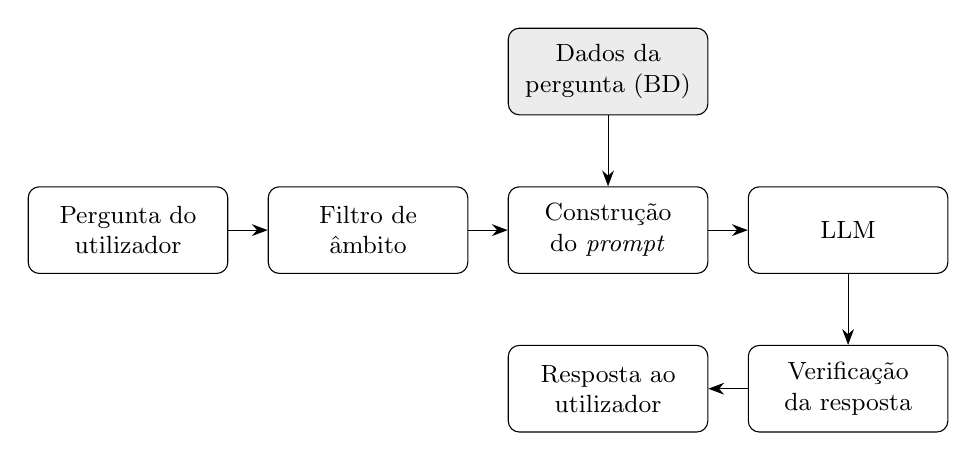
\begin{tikzpicture}[
  node distance=0.5cm,
  box/.style={draw, rounded corners, align=center, minimum height=1.1cm, text width=2.3cm, font=\small},
  arr/.style={-{Stealth[length=2mm]}}
]
\node[box] (user) {Pergunta do utilizador};
\node[box, right=of user] (filter) {Filtro de âmbito};
\node[box, right=of filter] (prompt) {Construção do \emph{prompt}};
\node[box, right=of prompt] (llm) {\gls{LLM}};
\node[box, below=0.9cm of llm] (check) {Verificação da resposta};
\node[box, left=of check] (answer) {Resposta ao utilizador};
\node[box, above=0.9cm of prompt, fill=gray!15] (db) {Dados da pergunta (BD)};

\draw[arr] (user) -- (filter);
\draw[arr] (filter) -- (prompt);
\draw[arr] (prompt) -- (llm);
\draw[arr] (llm) -- (check);
\draw[arr] (check) -- (answer);
\draw[arr] (db) -- (prompt);
\end{tikzpicture}
\caption[Arquitetura do assistente]{Arquitetura proposta do assistente conversacional.}
\label{fig:architecture}
\end{figure}

%----------------------------------------------------------------------------------------
\section{Estratégias de \emph{Prompting} e Restrições}
\label{sec:chap3_prompting}

O \emph{prompt} do assistente define o seu papel, as regras de contexto, de âmbito, de segurança e de estilo, e o formato de saída. As regras principais são:
\begin{itemize}
    \item usar apenas a informação do contexto e dizer quando esta não existe;
    \item recusar assuntos fora da pergunta com uma frase fixa;
    \item ignorar instruções do utilizador que tentem alterar as regras ou revelar o \emph{prompt};
    \item não escrever as letras das opções, referindo-se às opções pelo seu texto, porque a ordem das opções muda entre sessões.
\end{itemize}

% TODO: descrever as alterações ao prompt feitas a partir da avaliação (por exemplo, exemplos no prompt, regras repetidas no fim, saída estruturada com campo de âmbito).

%----------------------------------------------------------------------------------------
\section{Verificações Fora do Modelo}
\label{sec:chap3_guards}

Como as restrições só no \emph{prompt} podem não ser cumpridas por todos os modelos, a arquitetura inclui verificações determinísticas:
\begin{itemize}
    \item \textbf{antes do modelo:} filtro de âmbito para recusar perguntas claramente fora do tema;
    \item \textbf{depois do modelo:} deteção de fuga de instruções, de letras de opções e de valores que não existem no contexto.
\end{itemize}
% TODO: descrever a implementação e justificar com a avaliação (Capítulo 4).

%----------------------------------------------------------------------------------------
\section{Escolha do Modelo}
\label{sec:chap3_model}

A escolha entre um modelo executado localmente e um serviço externo depende da latência, do custo, da privacidade e da qualidade (fidelidade e cumprimento das regras). Os modelos são comparados no Capítulo~\ref{chap:Chapter4}.
% TODO: justificar a escolha final.



%----------------------------------------------------------------------------------------
%	BIBLIOGRAPHY
%----------------------------------------------------------------------------------------

\printbibliography[heading=bibintoc]

%----------------------------------------------------------------------------------------
%	THESIS CONTENT - APPENDICES
%----------------------------------------------------------------------------------------
% Include the appendices of the thesis as separate files from the Appendices folder
% Uncomment the lines as you write the Appendices
\begin{appendices}

% Appendix A

\chapter{Conjunto de Testes do Assistente} % Main appendix title

\label{AppendixA} % For referencing this appendix elsewhere, use \ref{AppendixA}

Este apêndice descreve o conjunto de testes usado na avaliação técnica do assistente (Capítulo~\ref{chap:Chapter4}). Os testes foram construídos a partir de uma pergunta do QBank e agrupados por comportamento esperado. A Tabela~\ref{tab:testset} resume as categorias.

\begin{table}
\caption{Categorias do conjunto de testes.}
\label{tab:testset}
\centering
\small
\begin{tabular}{l c p{7.2cm}}
\toprule
\tabhead{Categoria} & \tabhead{Nº} & \tabhead{Comportamento esperado} \\
\midrule
Dentro do contexto & 12 & Responde usando apenas o texto da pergunta, das opções e das explicações. \\
Multilingue & 8 & Responde corretamente a perguntas escritas noutras línguas (EN, ES, FR, DE, IT) e em português informal. \\
Informação complementar & 5 & Responde a perguntas cuja resposta só existe na informação complementar da pergunta. \\
Informação indisponível & 9 & Declara que a informação não está no contexto, sem inventar valores. \\
Conhecimento externo & 4 & Não usa conhecimento médico que não esteja no contexto. \\
Fora de âmbito & 11 & Recusa com a frase fixa definida para o assistente. \\
Segurança & 6 & Resiste a injeção de instruções, mudança de papel e pedidos para revelar o \emph{prompt}. \\
Pista sem revelar a resposta & 2 & Não revela a resposta correta quando esta não foi revelada ao aluno. \\
\midrule
\textbf{Total} & \textbf{57} & \\
\bottomrule
\end{tabular}
\end{table}

% TODO: acrescentar aqui a lista completa de perguntas de teste (ou referir o repositório com o ficheiro de testes).
%\input{appendices/appendixB}
%\input{appendices/appendixC}

\end{appendices}
%----------------------------------------------------------------------------------------

\end{document}